%% LyX 2.2.3 created this file.  For more info, see http://www.lyx.org/.
%% Do not edit unless you really know what you are doing.
\documentclass[12pt,english]{article}
\usepackage[T1]{fontenc}
\usepackage[latin9]{inputenc}
\usepackage[letterpaper]{geometry}
\geometry{verbose,tmargin=1in,bmargin=1in,lmargin=1in,rmargin=1in}
\usepackage{float}
\usepackage{url}
\usepackage{amstext}
\usepackage{graphicx}

\makeatletter
\@ifundefined{showcaptionsetup}{}{%
 \PassOptionsToPackage{caption=false}{subfig}}
\usepackage{subfig}
\makeatother

\usepackage{babel}
\begin{document}

\title{The MiniWeather Mini App}

\author{Matt Norman, Oak Ridge National Laboratory}

\date{~}

\maketitle
\tableofcontents{}

\section{Introduction}

The miniWeather code mimics the basic dynamics seen in atmospheric
weather and climate. The dynamics themselves are dry compressible,
stratified, non-hydrostatic flows dominated by buoyant forces that
are relatively small perturbations on a hydrostatic background state.
The equations in this code themselves form the backbone of pretty
much all fluid dynamics codes, and this particular flavor forms the
base of all weather and climate modeling.

With about 500 total lines of code (and only about 200 lines that
you care about), it serves as an approachable place to learn parallelization
and porting using MPI + X, where X is OpenMP, OpenACC, CUDA, or potentially
other approaches to CPU and accelerated parallelization. The code
uses periodic boundary conditions in the $x$-direction and solid
wall boundary conditions in the $z$-direction. 

\subsection{Brief Description of the Code}

\subsubsection{Domain Parameters}

A fuller description of the science, math, and dynamics are play are
in Section \ref{sec:Physics,-PDEs,-and}, but this section is reserved
to describing some of the main variables and flow in the code. The
code is decomposed in two spatial dimensions, $x$ and $z$, with
\texttt{nx\_glob} and \texttt{nz\_glob} cells in the global domain
and \texttt{nx} and \texttt{nz} cells in the local domain, using straightforward
domain decomposition for MPI-level parallelization. The global domain
is of size \texttt{xlen} and \texttt{zlen} meters, and \texttt{hs}
``halo'' cells are appended to both sides of each dimension for
convenience in forming stencils of cells for reconstruction.

\subsubsection{Fluid State Variables}

There are four main arrays used in this code: \texttt{state}, \texttt{state\_tmp},
\texttt{flux}, and \texttt{tend}, and the dimensions for each are
given in the code upon declaration in the comments. Each of these
arrays is described briefly below:
\begin{itemize}
\item \texttt{state}: This is the fluid state at the current time step,
and it is the only array that persists from one time step to the next.
The other four are only used within the calculations to advance the
model to the next time step. The fluid state describes the \emph{average}
state over each cell area in the spatial domain. This variable contains
four fluid states, which are the traditional mass, momenta, and thermodynamic
quantities of most fluid models:
\begin{enumerate}
\item Density (\texttt{ID\_DENS}): The 2-D density of the fluid in $\text{kg}\,\text{m}^{-2}$
(note this is normally $\text{kg}\,\text{m}^{-3}$, but this is a
2-D model, not 3-D)
\item U-momentum (\texttt{ID\_UMOM}): The momentum per unit area of the
fluid in the $x$-direction calculated as $\rho u$, where $u$ is
the $x$-direction wind velocity. The units are $\text{kg}\,\text{m}^{-1}\,\text{s}^{-1}$.
Note that to get true momentum, you must integrate over the cell.
\item W-momentum (\texttt{ID\_WMOM}): The momentum per unit area of the
fluid in the $z$-direction calculated as $\rho w$, where $w$ is
the $w$-direction wind velocity. The units are $\text{kg}\,\text{m}^{-1}\,\text{s}^{-1}$.
Note that to get true momentum, you must integrate over the cell.
\item Potential Temperature (\texttt{ID\_RHOT}): The product of density
and potential temperature, $\rho\theta$, where $\theta=T\left(P_{0}/P\right)^{R_{d}/c_{p}}$,
$P_{0}=10^{5}\,\text{Pa}$, $T$ is the true temperature, and $R_{d}$
and $c_{p}$ are the dry air constant and specific heat at constant
pressure for dry air, respectively. The units of this quantity are
$\text{K}\,\text{kg}\,\text{m}^{-2}$.
\end{enumerate}
\item \texttt{state\_tmp}: This is a temporary copy of the fluid state used
in the Runge-Kutta integration to keep from overwriting the state
at the beginning of the time step, and it has the same units and meaning.
\item \texttt{flux}: This is fluid state at cell boundaries in the $x$-
and $z$-directions, and the units and meanings are the same as for
\texttt{state} and \texttt{state\_tmp}. In the $x$-direction update,
the values of \texttt{flux} at indices \texttt{i} and \texttt{i+1}
represents the fluid state at the left- and right-hand boundaries
of cell \texttt{i}. The indexing is analagous in the $z$-direction.
The fluxes are used to exchange fluid properties with neighboring
cells.
\item \texttt{tend}: This is the time tendency of the fluid state $\partial\mathbf{q}/\partial t$,
where $\mathbf{q}$ is the the \texttt{state} vector, and as the name
suggests, it has the same meaning and units as \texttt{state}, except
per unit time (appending $\text{s}^{-1}$ to the units). In the Finite-Volume
method, the time tendency of a cell is equivalent to the divergence
of the flux across a cell.
\end{itemize}

\subsubsection{Overal Model Flow}

This code follows a traditional Finite-Volume control flow.

To compute the time tendency, given an initial state at the beginning
of a time step that contains cell-averages of the fluid state, the
value of the state at cell boundaries is reconstructed using a stencil.
Then, a viscous term is added to the fluid state at the cell boundaries
to improve stability. Next, the tendencies are computed as the divergence
of the flux across the cell. Finally, the tendencies are applied to
the fluid state.

Once the time tendency is computed, the fluid PDEs are essentially
now cast as a set of ODEs varying only in time, and this is called
the ``semi-discretized'' form of the equations. To solve the equations
in time, an ODE solver is used, in this case, a Runge-Kutta method.
Finally, at the highest level, the equations are split into separate
solves in each dimension, $x$ and $z$.

\section{Compiling and Running the Code}

\subsection{Required Libraries}

To run everything in this code, you need MPI, parallel-netcdf, ncview,
and an OpenACC compiler (preferably PGI 17+) to be installed. The
serial code still uses MPI because I figured it was best to start
with parallel I/O in place so that it's ready to go when the MPI implementation
is done. 

You can download parallel-netcdf from:\\
\url{https://trac.mcs.anl.gov/projects/parallel-netcdf}\\
Also, you can download a free version of PGI Community Edition (which
has OpenACC implemented) from:\\
\url{https://www.pgroup.com/products/community.htm}\\
You'll probably also want to have ``ncview'' installed so you can
easily view the NetCDF files. Ncview also makes it easy to see a movie
of the solution as it evolves in time:\\
\url{http://meteora.ucsd.edu/~pierce/ncview_home_page.html}

\subsection{Directories and Compiling}

There are three main directories in the mini app: (1) a Fortran source
directory; (2) a C source directory; and (3) a documentation directory,
which you presumably know about because it contains this text you're
reading now. The C code is technically C++ code but only because I
wanted to use the ampersand pass by reference notation.

To compile the code, first edit the Makefile and change the flags
to point to your parallel-netcdf installation as well as change the
flags based on which compiler you are using. There are four versions
of the code: serial, mpi, mpi+openmp, and mpi+openacc. The filenames
make it clear which file is associated with which programming paradigm.
To make all of these at once, simply type ``make''. To make them
individually, you can type ``make serial'', ``make mpi'', ``make
openmp'', and ``make openacc''.

\subsection{Altering the Code's Configurations}

There are four aspects of the configuration you can edit easily, and
they are clearly labeled in the code as ``USER-CONFIGURABLE PARAMETERS''.
These include: (1) the number of cells to use {[}``nx\_glob'' and
``nz\_glob''{]}; (2) the amount of time to simulate {[}``sim\_time''{]};
(3) the frequency to output data to file {[}``output\_freq''{]};
and (4) the initial data to use {[}``data\_spec\_int''{]}. 

\subsection{Running the Code}

To run the code, simply call ``mpirun -n {[}\# ranks{]} ./mini\_weather\_{[}version{]}''.
Since parameters are set in the code itself, you don't need to pass
any parameters. Some machines use different tools instead of mpirun
(e.g., OLCF's Titan uses ``aprun'').

\subsection{Viewing the Output}

The file I/O is done in the netCDF format: (\url{https://www.unidata.ucar.edu/software/netcdf/}).
To me, the easiest way to view the data is to use a tool called ``ncview''
(\url{http://meteora.ucsd.edu/~pierce/ncview_home_page.html}). To
use it, you can simply type ``ncview output.nc'', making sure you
have X-forwarding enabled in your ssh session. Further, you can call
``ncview -frames output.nc'', and it will dump out all of your frames
in the native resolution you're viewing the data in, and you you can
render a movie with tools like ffmpeg. 

\section{Parallelization}

This code was designed to parallelize with MPI first and then OpenMP
or OpenACC next, but you can always parallelize with OpenMP or OpenACC
without MPI if you want. But it is rewarding to be able to run it
on multiple nodes at higher resolution for more and sharper eddies
in the dynamics. 

As you port the code, you'll want to change relatively little code
at a time, re-compile, re-run, and look at the output to see that
you're still getting the right answer. There are advantages to using
a visual tool to check the answer, as it can sometimes give you clues
as to why you're not getting the right answer. 

Note that you only need to make changes code within the first 450
source lines. Everything below that is initialization and I/O code
that doesn't need to be parallelized (unless you want to). There's
a note in the serial code that tells you at what point the rest of
the code will remain the same, even after parallelization.

\subsection{Indexing}

The code makes room for so-called ``halo'' cells in the fluid state.
This is a common practice in any algorithm that uses stencil-based
reconstruction to estimate variation within a domain. In this code,
there are ``hs'' halo cells on either side of each dimension, and
I pretty much hard-code hs=2.

\subsubsection{Fortran}

In the Fortran code's fluid state (``state''), the x- and z-dimensions
are dimensioned as multi-dimensional arrays that range from 1-hs:nx+hs.
In the x-direction, 1-hs:0 belong to the MPI task to the left, cells
1:nx belong to the current MPI task, and nx+1:nx+hs belong to the
MPI task to the right. In the z-dimension, 1-hs:0 are artificially
set to mimic a solid wall boundary condition at the bottom, and nz+1:nz+hs
are the same for the top boundary. The cell-interface fluxes (``flux'')
are dimensioned as 1:nx+1 and 1:nz+1 in the x- and z-directions, and
the cell average tendencies (``tend'') are dimensioned 1:nx and
1:nz in the x- and z-directions. The cell of index i will have left-
and right-hand interface fluxes of index i and i+1, respectively,
and it will be evolved by the tendency at index i. The analog of this
is also true in the z-direction.

\subsubsection{C}

In the C code, the fluid state array is dimensioned to size (nz+2{*}hs)
and (nx+2{*}hs) in the x- and z-directions. In the x-direction, cells
0 to hs-1 belong to the left MPI task, cells hs to nx+hs-1 belong
to the current MPI taks, and cells nx+hs to nx+2{*}hs-1 belong to
the right MPI task. The z-direction's halo cells are used to mimic
solid wall boundaries. The cell-interface fluxes (``flux'') are
dimensioned as nx+1 and nz+1 in the x- and z-directions, and the cell
average tendencies (``tend'') are dimensioned nx and nz in the x-
and z-directions. The cell of index i+hs will have left- and right-hand
interface fluxes of index i and i+1, respectively, and it will be
evolved by the tendency at index i.The analog of this is also true
in the z-direction.

\subsection{MPI}

This code was designed to use domain decomposition, where each MPI
rank ``owns'' a certain set of cells in the x-direction and contains
two ``halo'' cells from the left- and right-hand MPI tasks in the
x-direction as well. The domain is only decomposed in the $x$-direction
and not the $z$-direction.

IMPORTANT: Please be sure to set ``nranks'', ``myrank'', ``nx'',
``i\_beg'', ``left\_rank'', and ``right\_rank''. These are clearly
marked in the serial source code. You can set more variables, but
these are used elsewhere in the code (particularly in the parallel
file I/O), so they must be set.

To parallelize with MPI, there are only two places in the code that
need to be altered. The first is the initialization, a subroutine
/ function named ``init'', where you must determine the number of
ranks, you process's rank, the beginning index of your rank's first
cell in the x-direction, the number of x-direction cells your rank
will own, and the MPI rank IDs that are to your left and your right.
Because the code is periodic in the $x$-direction, your left and
right neighboring ranks will wrap around. For instance, if your are
rank zero, your left-most rank will be nranks-1.

The second place is in the routine that sets the halo values in the
$x$-direction. In this routine, you need to:
\begin{enumerate}
\item Create MPI data buffers (at the same place the other arrays are declared)
to hold the data that needs to be sent and received, allocate them
in the init() routine, and deallocate them in the finalize() routine.
\item Pack the data you need to send to your left and right MPI neighbors
\item Send the data to your left and right MPI neighbors
\item Receive the data from your left and right MPI neighbors
\item Unpack the data from your left and right neighbors and place the data
into your MPI rank's halo cells. 
\end{enumerate}
Once you complete this, the code will be fully parallelized in MPI.
Both of the places you need to add code for MPI are marked in the
serial code, and there are some extra hints in the ``set\_halo\_values\_x()''
routine as well.

\subsection{OpenMP}

For the OpenMP code, you basically need to decorate the loops with
``omp parallel do'' or ``omp parallel for'' and pay attention
to any variables you need to make ``private'' so that each thread
has its own copy. Keep in mind that OpenMP works best on ``outer''
loops rather than ``inner'' loops. Also, for sake of performance,
there are a couple of instances where it is wise to use the ``collapse''
clause because the outermost loop is not large enough to support the
number of threads most CPUs have.

\subsection{OpenACC}

The OpenACC approach will differ depending on whether you're in Fortran
or C. Just a forewarning, OpenACC is much more convenient in Fortran
when it comes to data movement because in Fortran, the compiler knows
how big your arrays are, and therefore the compiler can (and does)
create all of the data movement for you. All you have to do is optimize
the data movement after the fact.

\subsubsection{Fortran Code}

The OpenACC parallelization is a bit more involved when it comes to
performance. But, it's a good idea to just start with the kernels
themselves, since the compiler will generate all of your data statements
for you on a per-kernel basis. You need to pay attention to private
variables here as well.

Once you're getting the right answer with the kernels on the GPU,
you can look at optimizing data movement by putting in data statements.
I recommend putting data statements for the state, tend, flux, hy\_{*},
and the MPI buffers around the main time stepping loop. Then, you
need to move the data to the host before sending MPI data, back to
the device once you receive MPI data, and to the host before file
I/O.

\subsubsection{C Code}

In the C code, you'll need to put in manual copy, copyin, and copyout
statements on a per-kernel basis, and you'll need to explicitly declare
the size of each array as well. Other than this, the approach is the
same as with the Fortran case. Once you have your kernels ported,
you can optimize the data movement by wrapping the main time stepping
loop in data statements, making sure the host has the data for I/O
and sending MPI buffers and the device has the data after receiving
MPI buffers.

\section{Numerical Experiments}

A number of numerical experiments are in the code for you to play
around with. You can set these by changing the ``data\_spec\_int''
variable. 

\subsection{Rising Thermal}

data\_spec\_int = DATA\_SPEC\_THERMAL\\
sim\_time = 1000\\
This simulates a rising thermal in a neutral atmosphere, which will
look something like a ``mushroom'' cloud (without all of the violence).

\begin{figure}[H]
\begin{centering}
\subfloat[500s]{\begin{centering}
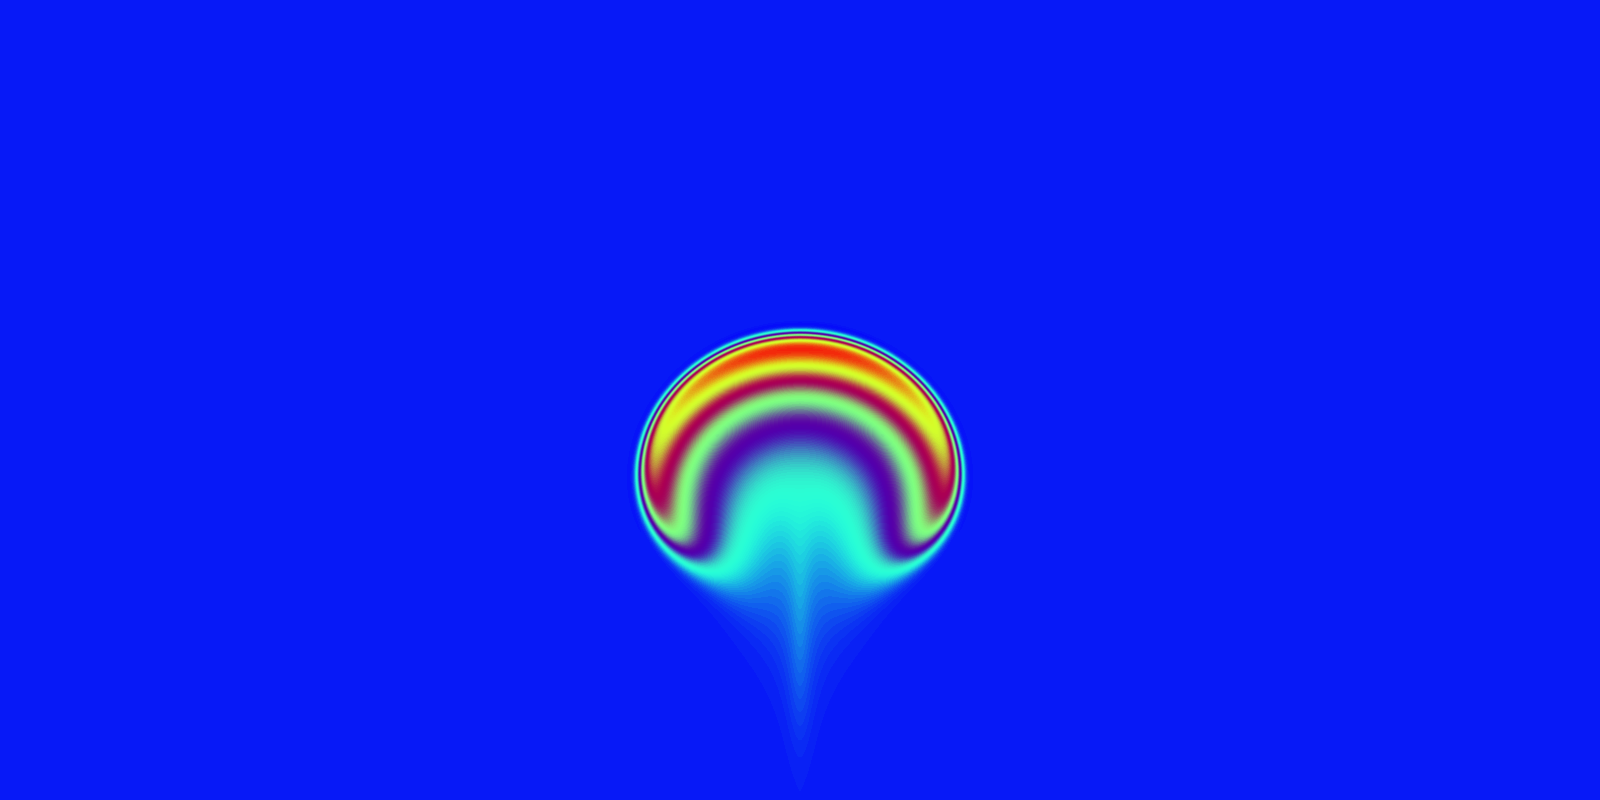
\includegraphics[width=3in]{images/thermal_pt_0500}
\par\end{centering}
}\subfloat[1,000s]{\begin{centering}
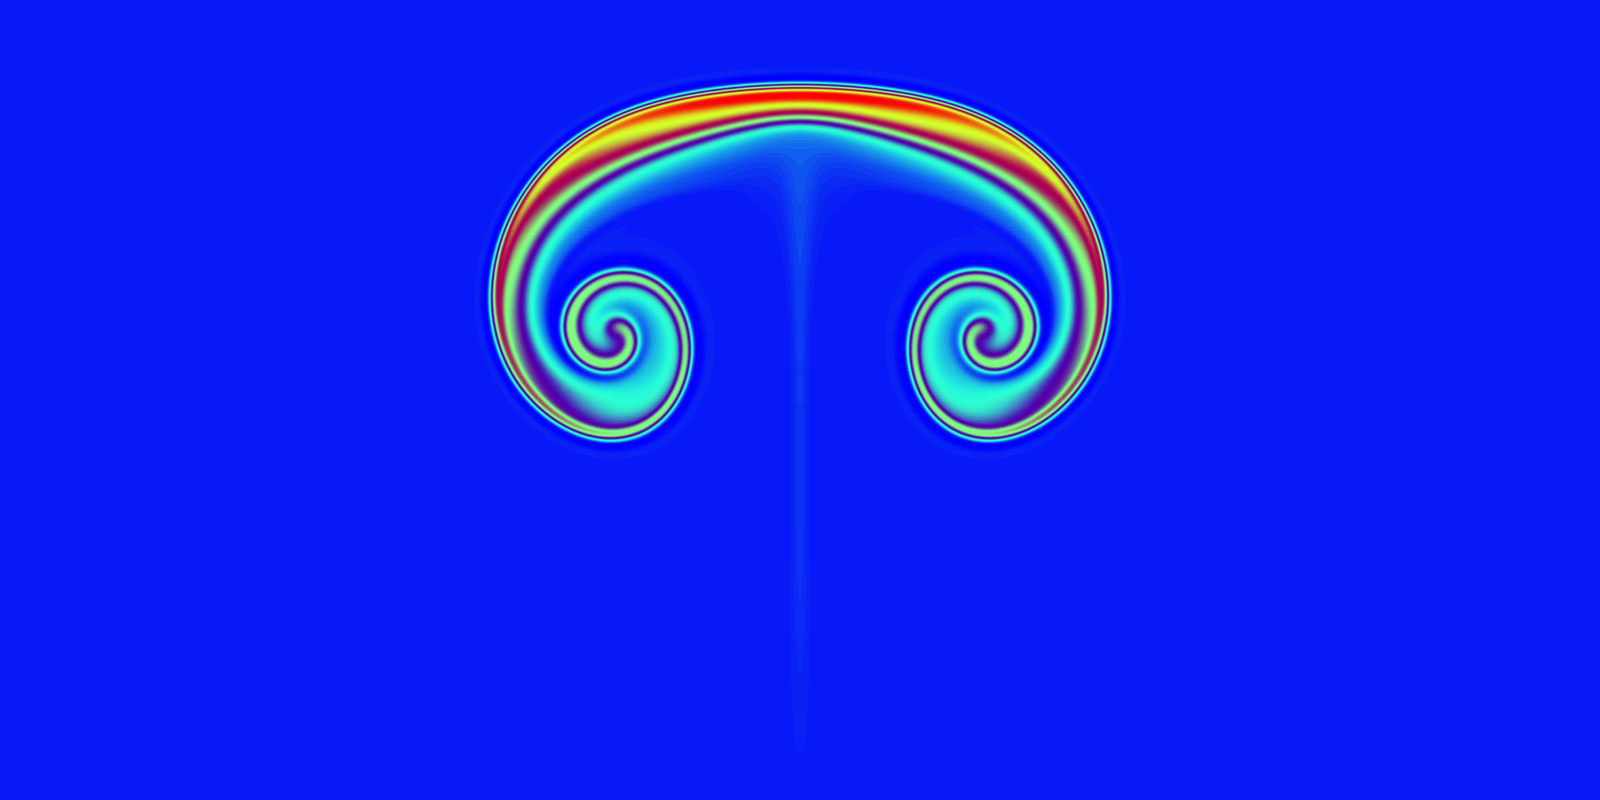
\includegraphics[width=3in]{images/thermal_pt_1000}
\par\end{centering}
}
\par\end{centering}
\caption{Rising Thermal test case: Potential Temperature perturbation with
1600x800 cells.}
\end{figure}

\subsection{Colliding Thermals}

data\_spec\_int = DATA\_SPEC\_COLLISION\\
sim\_time = 600\\
This is similar to the rising thermal test case except with a cold
bubble at the model top colliding with a warm bubble at the model
bottom to produce some cool looking eddies. This test case is mainly
for looks, not physics.

\begin{figure}[H]
\begin{centering}
\subfloat[200s]{\begin{centering}
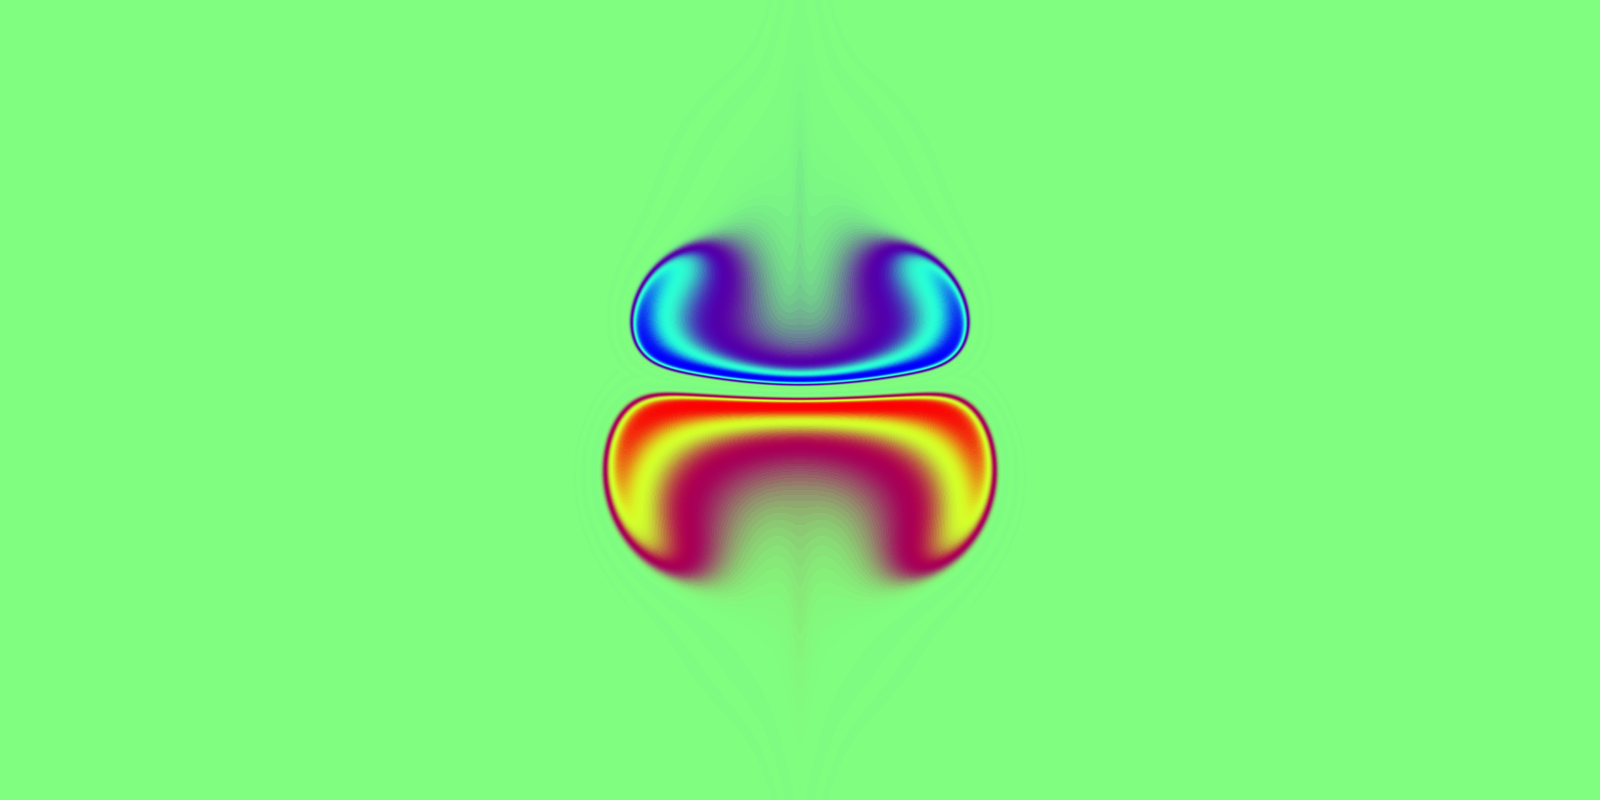
\includegraphics[width=3in]{images/collision_pt_0200}
\par\end{centering}
}\subfloat[400s]{\begin{centering}
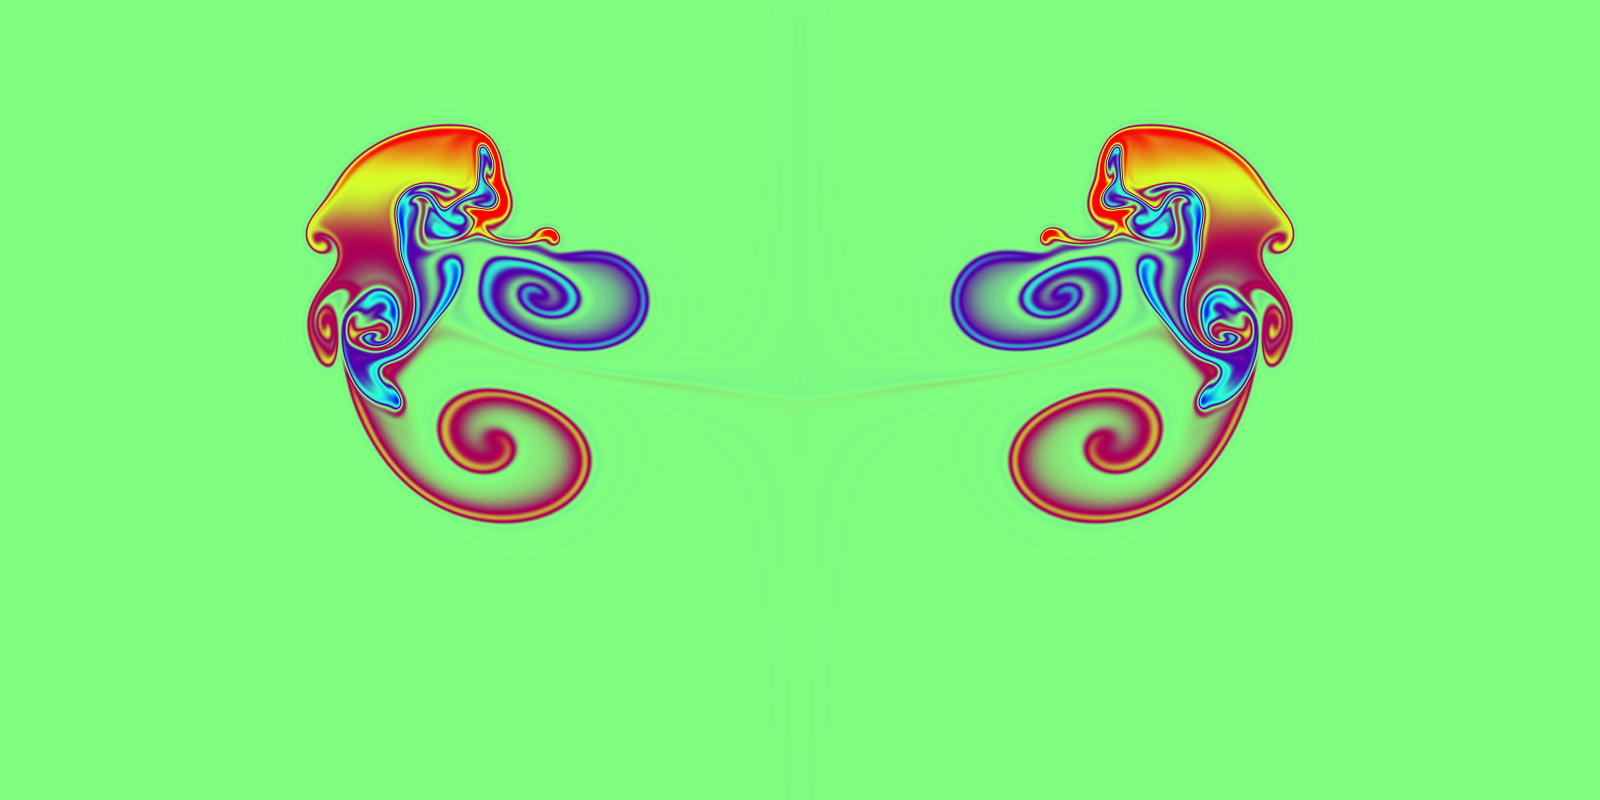
\includegraphics[width=3in]{images/collision_pt_0400}
\par\end{centering}
}
\par\end{centering}
\begin{centering}
\subfloat[700s]{\begin{centering}
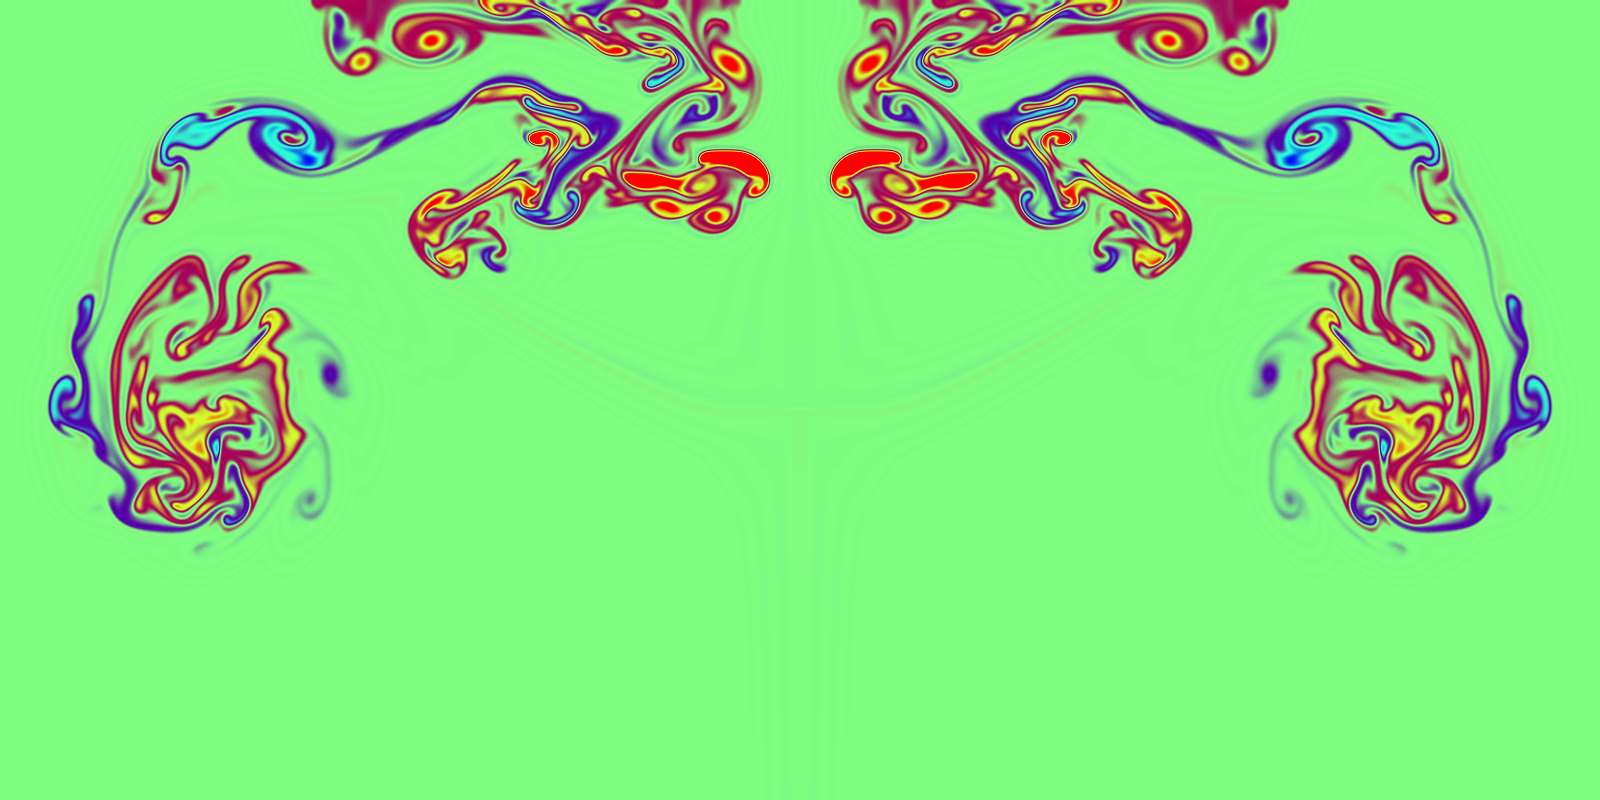
\includegraphics[width=3in]{images/collision_pt_0700}
\par\end{centering}
}
\par\end{centering}
\caption{Colliding Thermals test case: Potential Temperature perturbation with
1600x800 cells.}
\end{figure}

\subsection{Mountain Gravity Waves}

data\_spec\_int = DATA\_SPEC\_MOUNTAIN\\
sim\_time = 1500\\
This test cases passes a horizontal wind over a faked mountain at
the model bottom in a stable atmosphere to generate a train of stationary
gravity waves across the model domain.

\begin{figure}[H]
\begin{centering}
\subfloat[400s]{\begin{centering}
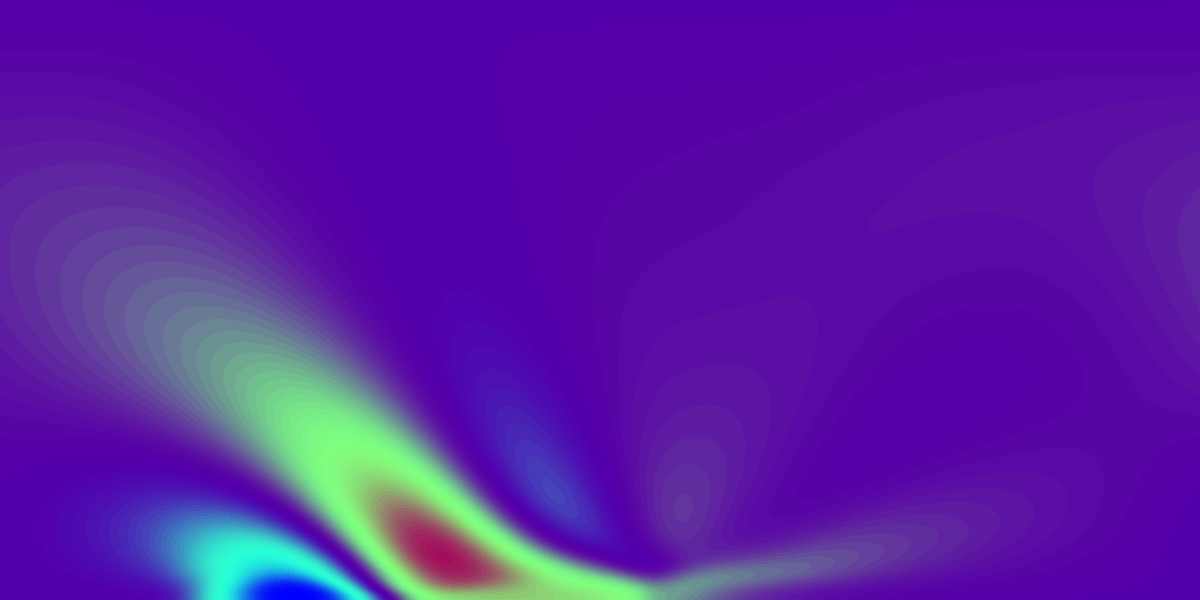
\includegraphics[width=3in]{images/mountain_pt_0400}
\par\end{centering}
}\subfloat[1,300s]{\begin{centering}

\includegraphics[width=3in]{images/mountain_pt_1300}
\par\end{centering}
}
\par\end{centering}
\caption{Mountain Gravity Waves test case: Potential Temperature perturbation
with 400x200 cells.}
\end{figure}

\subsection{Density Current}

data\_spec\_int = DATA\_SPEC\_DENSITY\_CURRENT\\
sim\_time = 600\\
This test case creates a neutrally stratified atmosphere with a strong
cold bubble in the middle of the domain that crashes into the ground
to give the feel of a weather front (more of a downburst, really).

\begin{figure}[H]
\begin{centering}
\subfloat[200s]{\begin{centering}
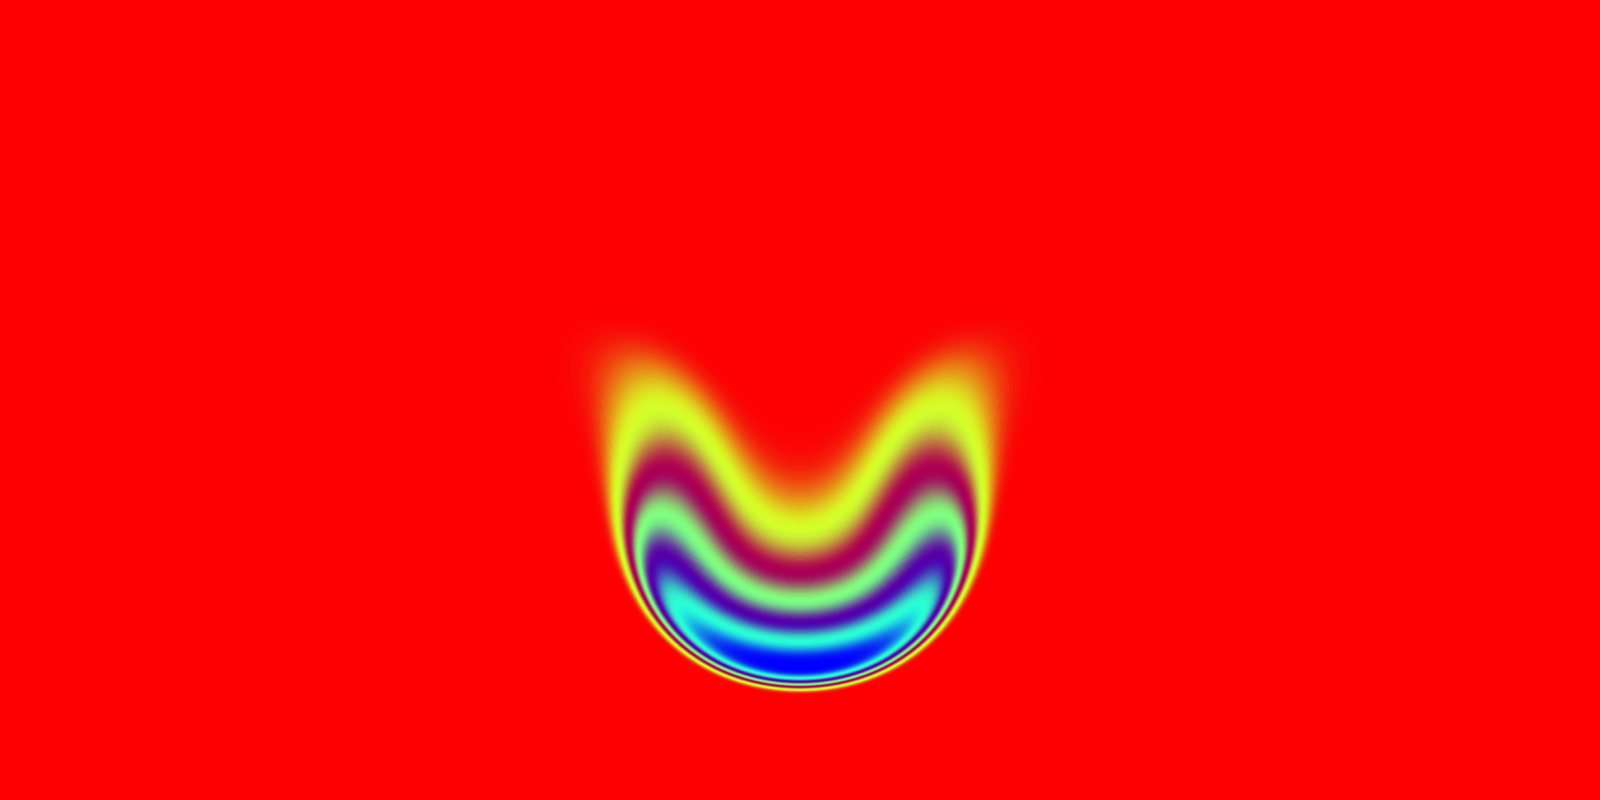
\includegraphics[width=3in]{images/density_current_pt_0200}
\par\end{centering}
}\subfloat[600s]{\begin{centering}

\includegraphics[width=3in]{images/density_current_pt_0600}
\par\end{centering}
}
\par\end{centering}
\caption{Density Current test case: Potential Temperature perturbation with
1600x800 cells.}
\end{figure}

\subsection{Injection}

data\_spec\_int = DATA\_SPEC\_INJECTION\\
sim\_time = 1200\\
A narrow jet of fast and slightly cold wind is injected into a balanced,
neutral atmosphere at rest from the left domain near the model top.
This has nothing to do with atmospheric flows. It's just here for
looks. 

\begin{figure}[H]
\begin{centering}
\subfloat[300s]{\begin{centering}

\includegraphics[width=3in]{images/injection_pt_0300}
\par\end{centering}
}\subfloat[1,000s]{\begin{centering}

\includegraphics[width=3in]{images/injection_pt_1000}
\par\end{centering}
}
\par\end{centering}
\caption{Injection test case: Potential Temperature perturbation with 1600x800
cells.}
\end{figure}

\section{Physics, PDEs, and Numerical Approximations\label{sec:Physics,-PDEs,-and}}

I put this section last just for the sake of completion in case you're
curious what's actually going on in the code. While the numerical
approximations in this code are certainly cheap and dirty, they are
a fast and easy way to get the job done in a relatively small amount
of code. For instance, on 16 K20x GPUs, you can perform a ``colliding
thermals'' simulation with 5 million grid cells (3200 $\times$ 1600)
in just a few minutes.

\subsection{The 2-D Euler Equations}

This app simulates the 2-D inviscid Euler equations for stratified
fluid dynamics, which are defined as follows: 
\begin{equation}
\frac{\partial}{\partial t}\left[\begin{array}{c}
\rho\\
\rho u\\
\rho w\\
\rho\theta
\end{array}\right]+\frac{\partial}{\partial x}\left[\begin{array}{c}
\rho u\\
\rho u^{2}+p\\
\rho uw\\
\rho u\theta
\end{array}\right]+\frac{\partial}{\partial z}\left[\begin{array}{c}
\rho w\\
\rho wu\\
\rho w^{2}+p\\
\rho w\theta
\end{array}\right]=\left[\begin{array}{c}
0\\
0\\
-\rho g\\
0
\end{array}\right]\label{eq:equations_spelled_out}
\end{equation}
\[
\rho_{H}=-\frac{1}{g}\frac{\partial p}{\partial z}
\]
where $\rho$ is density, $u$, and $w$ are winds in the $x$-, and
$z$-directions, respectively, $\theta$ is potential temperature
related to temperature, $T$, by $\theta=T\left(P_{0}/P\right)^{R_{d}/c_{p}}$,
$P_{0}=10^{5}\,\text{Pa}$ is the surface pressure, $g=9.8\text{\,\ m}\,\mbox{s}^{-2}$
is acceleration due to gravity, $p=C_{0}\left(\rho\theta\right)^{\gamma}$
is the pressure as determined by an alternative form of the ideal
gas equation of state, $C_{0}=R_{d}^{\gamma}p_{0}^{-R_{d}/c_{v}}$,
$R_{d}=287\,\mbox{J}\,\mbox{kg}^{-1}\,\mbox{K}^{-1}$ is the dry gas
constant, $\gamma=c_{p}/c_{v}$, $c_{p}=1004\,\mbox{J}\,\mbox{kg}^{-1}\,\mbox{K}^{-1}$
is specific heat at constant pressure, and $c_{v}=717\,\mbox{J}\,\mbox{kg}^{-1}\,\mbox{K}^{-1}$
is specific heat at constant volume. This can be cast in a more convenient
form as:
\begin{equation}
\frac{\partial\mathbf{q}}{\partial t}+\frac{\partial\mathbf{f}}{\partial x}+\frac{\partial\mathbf{h}}{\partial z}=\mathbf{s}\label{eq:dynamics_definition}
\end{equation}
where a bold font represents a vector quantity.

\subsection{Maintaining Hydrostatic Balance}

The flows this code simulates are relatively small perturbations off
of a ``hydrostatic'' balance, which balances gravity with a difference
in pressure:
\[
\frac{dp}{dz}=-\rho g
\]
Because small violations of this balance lead to significant noise
in the vertical momentum, it's best not to try to directly reconstruct
this balance but rather to only reconstruct the perturbations. Therefore,
hydrostasis is subtracted from (\ref{eq:equations_spelled_out}) to
give:
\begin{equation}
\frac{\partial}{\partial t}\left[\begin{array}{c}
\rho^{\prime}\\
\rho u\\
\rho w\\
\left(\rho\theta\right)^{\prime}
\end{array}\right]+\frac{\partial}{\partial x}\left[\begin{array}{c}
\rho u\\
\rho u^{2}+p\\
\rho uw\\
\rho u\theta
\end{array}\right]+\frac{\partial}{\partial z}\left[\begin{array}{c}
\rho w\\
\rho wu\\
\rho w^{2}+p^{\prime}\\
\rho w\theta
\end{array}\right]=\left[\begin{array}{c}
0\\
0\\
-\rho^{\prime}g\\
0
\end{array}\right]\label{eq:equations_spelled_out_no_hydrostasis}
\end{equation}
where a ``prime'' quantity represents that variable with the hydrostatic
background state subtracted off.

\subsection{Dimensional Splitting}

This equation is solved using dimensional splitting for simplicity
and speed. The equations are split into $x$- and $z$-direction solves
that are, respectively:
\[
x:\,\,\,\,\,\,\,\,\,\,\frac{\partial\mathbf{q}}{\partial t}+\frac{\partial\mathbf{f}}{\partial x}=\mathbf{0}
\]
\[
z:\,\,\,\,\,\,\,\,\,\,\frac{\partial\mathbf{q}}{\partial t}+\frac{\partial\mathbf{h}}{\partial x}=\mathbf{s}
\]
Each time step, the order in which the dimensions are solved is reversed,
giving second-order accuracy overall. 

\subsection{Finite-Volume Spatial Discretization\label{subsec:Finite-Volume-Spatial-Discretiza}}

A Finite-Volume discretization is used in which the PDE in a given
dimension is integrated over a cell domain, $\Omega_{i}\in\left[x_{i-1/2},x_{i+1/2}\right]$,
where $x_{i\pm1/2}=x_{i}\pm\Delta x$, $x_{i}$ is the cell center,
and $\Delta x$ is the width of the cell. The integration is the same
in the $z$-direction. Using the Gauss divergence theorem, this turns
the equation into (using the $z$-direction as an example):
\begin{equation}
\frac{\partial\overline{\mathbf{q}}_{i,k}}{\partial t}=-\frac{\mathbf{h}_{i,k+1/2}-\mathbf{h}_{i,k-1/2}}{\Delta z}+\overline{\mathbf{s}}_{i,k}\label{eq:fv_discretization}
\end{equation}
where $\overline{\mathbf{q}}_{i,k}$ and $\overline{\mathbf{s}}_{i,k}$
are the cell-average of the fluid state and source term over the cell
of index $i,k$.

To compute the update one needs the flux vector at the cell interfaces
and the cell-averaged source term. To compute the flux vector at interfaces,
fourth-order-accurate polynomial interpolation is used using the four
cell averages surrounding the cell interface in question.

\subsection{Runge-Kutta Time Integration}

The equation (\ref{eq:fv_discretization}) still has a time derivative
that needs integrating, and a simple low-storage Runge-Kutta ODE solver
is used to integrate the time derivative, and it is solved as follows:
\[
\mathbf{q}^{\star}=\mathbf{q}^{n}+\frac{\Delta t}{3}RHS\left(\mathbf{q}^{n}\right)
\]
\[
\mathbf{q}^{\star\star}=\mathbf{q}^{n}+\frac{\Delta t}{2}RHS\left(\mathbf{q}^{\star}\right)
\]
\[
\mathbf{q}^{n+1}=\mathbf{q}^{n}+\Delta tRHS\left(\mathbf{q}^{\star\star}\right)
\]
When it comes to time step stability, I simply assume the maximum
speed of propagation is $450\,\text{m}\,\text{s}^{-1}$, which basically
means that the maximum wind speed is assumed to be $100\,\text{m}\,\text{s}^{-1}$,
which is a safe assumption. I set the CFL value to 1.5 for this code.

\subsection{``Hyper-viscosity''}

The centered fourth-order discretization in Section \ref{subsec:Finite-Volume-Spatial-Discretiza}
is unstable as is and requires extra dissipation to damp out small-wavelength
energy that would otherwise blow up the simulation. This damping is
accomplished with a scale-selective fourth-order so-called ``hyper''-viscosity
that is defined as:
\[
\frac{\partial\mathbf{q}}{\partial t}+\frac{\partial}{\partial x}\left(-\kappa\frac{\partial^{3}\mathbf{q}}{\partial x^{3}}\right)=\mathbf{0}
\]
and this is also solved with the Finite-Volume method just like above.
The hyperviscosity constant is defined as:
\[
\kappa=-\beta\left(\Delta x\right)^{4}2^{-4}\left(\Delta t\right)^{-1}
\]
where $\beta\in\left[0,1\right]$ is a user-defined parameter to control
the strength of the diffusion, where a higher value gives more diffusion.
The parameter $\beta$ is not sensitive to the grid spacing, and it
seems that $\beta=0.25$ is generally enough to get rid of $2\Delta x$
noise contamination.
\end{document}
